\subsection{Detector designs}
\begin{frame}
	\frametitle{Detector designs}
	\begin{itemize}
% 		\setlength{\itemsep}{\fill}
		\item Investigation of two different detector designs
		\vspace*{5pt}
		\begin{itemize}
			\item \textbf{planar diamonds}
			\begin{itemize}
				\item exchange of material
			\end{itemize}
			\item \textbf{3D diamonds}
			\begin{itemize}
				\item new type of detector
			\end{itemize}
		\end{itemize}
	\end{itemize}
	\begin{figure}[htbp] 
		\begin{center}
			\begin{subfigure}{0.45\textwidth}  
				\centering 
				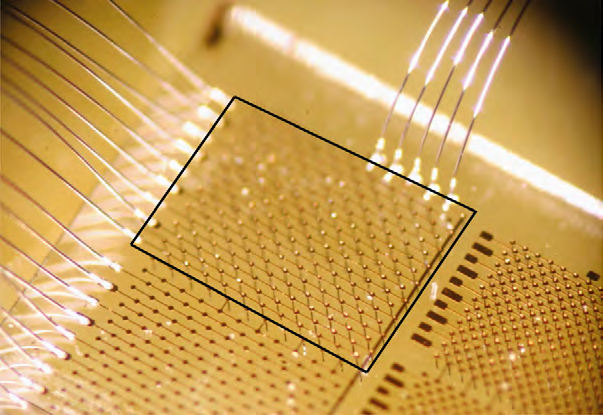
\includegraphics[height=0.4\textheight]{3D}
				\caption{prototype}
			\end{subfigure}
			\begin{subfigure}{0.45\textwidth} 
				\centering 
				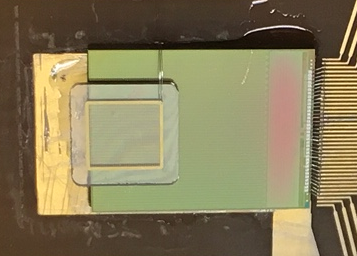
\includegraphics[height=0.4\textheight]{diapix}
				\caption{on CMS-Pixel chip} 	
				\label{fig:consecutive_cuts_lin} 
			\end{subfigure} 
			\caption{3D diamond detectors} 
			\label{fig:consecutive_cuts} 
		\end{center}
	\end{figure}
\end{frame}
% ============== new frame
\subsection{Detector material}
\begin{frame}
	\frametitle{Detector material}
	\begin{itemize}
		\setlength{\itemsep}{\fill}
		\item \textcolor{green}{$7-10$ times smaller charge loss due to radiation damage then in silicon}
		\item \textcolor{red}{signals (electrons created by a charged particle) two times smaller than in silicon}
		\item $\rightarrow$ diamond becoming superior than silicon at a certain irradiation
		\item other advantageous properties:
		\begin{itemize}
			\item isolating material \ra negligible leakage current \ra power saving 
			\item high thermal conductivity \ra heat spreader for electronics
			\item large band gap \ra no cooling required
			\item high charge carrier mobility \ra fast signals
			\item working principle like a solid state ionisation chamber \ra no pn-junction required
		\end{itemize}
		\item disadvantages:
		\begin{itemize}
			\item high price
			\item some not fully understood behaviours 
		\end{itemize}
	\end{itemize}
\end{frame}
% ============== new frame
\subsection{}
